\section{Refinement-based game semantics}

In this section we introduce the category $\mathcal{G}$ of games and strategies
we will use to interpret the behavior of low-level interacting components.

The objects of $\mathcal{G}$ are elementary games whose plays consists of
one question from the $\kw{O}$ followed by one answer from $\kw{P}$.
The morphisms $\sigma : A \rightarrow B$
are well-bracketed, alternating strategies for the game ${!A} \multimap {!B}$.
These restrictions ensures that no pointers or indices
are necessary to distinguish threads in a given play of the arrow game.

On the other hand,
our definition of strategy is generalized to accomodate specifications,
and $\mathcal{G}$ is equipped with a notion of refinement
suitable for our purposes.

\subsection{Games}

\subsubsection{Elementary games}

\begin{definition}
An \emph{elementary game} is given as a tuple
$A = \langle M_A^\kw{Q}, M_A^\kw{A}, W_{\!A},
       \preceq_A^\kw{Q}, \preceq_A^\kw{A} \rangle$, where
$M_A^\kw{Q}$ is a set of \emph{questions},
$M_A^\kw{A}$ is a set of \emph{answers}, and
$W_{\!A}$ is a set of \emph{worlds}.
The $W_{\!A}$-indexed relations
${\preceq}_A^\kw{Q} : \mathcal{R}_{W_{\!A}}(M_A^\kw{Q}, M_A^\kw{Q})$ and
${\preceq}_A^\kw{A} : \mathcal{R}_{W_{\!A}}(M_A^\kw{A}, M_A^\kw{A})$
define notions of \emph{refinement} for questions and answers.
\end{definition}

Elementary games proceed as follows:
$\kw{O}$ first chooses a question, then
$\kw{P}$ chooses an answer.
We can think of strategies for $A$ as partial functions
$\sigma : M_A^\kw{Q} \rightarrow \mathcal{P}^1(M_A^\kw{A})$
ordered by the simulation relation
$\Vdash {\preceq}_A^\kw{Q} \rightarrow \mathcal{P}^+({\preceq}_A^\kw{A})$.
Moreover,
we expect valid strategies to be self-simulating:
whenever $m_1 \preceq_A^\kw{Q} m_2$,
a valid strategy which reacts to the question $m_1$
with the answer $n_1$
will also react to the more general question $m_2$ ---
with an answer $n_2$ such that $n_1 \preceq_A^\kw{A} n_2$.

\subsubsection{Iterated games}

If we allow multiple iterations of the game,
the plays will be paths from $\kw{O}$ in the following graph:
\[
  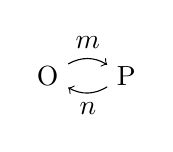
\begin{tikzpicture}[baseline=(O.base)]
    \node (O) at (0,0) {\kw{O}};
    \node (P) at (1,0) {\kw{P}};
    \path [->] (O) edge[bend left] node[auto] {$m$} (P);
    \path [->] (P) edge[bend left] node[auto] {$n$} (O);
  \end{tikzpicture}
  \qquad
  \begin{array}{c@{\,}l}
    m &\in M_A^\kw{Q} \\[1ex]
    n &\in M_A^\kw{A}
  \end{array}
\]
To formalize the relational aspects of iterations
of elementary games,
we can adjust the graph above so that its vertices are taken
from the set of worlds extended with a starting point $\star$,
and its edges are labelled by \emph{pairs} of related moves:
\[
  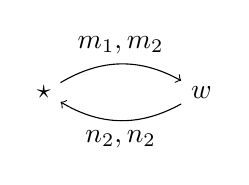
\begin{tikzpicture}[baseline=(O.base)]
    \node (O) at (0,0) {$\star$};
    \node (P) at (2,0) {$w$};
    \path [->] (O) edge[bend left] node[auto] {$m_1, m_2$} (P);
    \path [->] (P) edge[bend left] node[auto] {$n_2, n_2$} (O);
  \end{tikzpicture}
  \qquad
  \begin{array}{c}
    (m_1, m_2) \in {\preceq}_A^\kw{Q} \\[.5ex]
    w \in W_{\!A} + \star \\[.5ex]
    (n_1, n_2) \in {\preceq}_A^\kw{A}
  \end{array}
\]
Two sequences of moves $s_1, s_2$
are related at a world $w$
if the graph contains a path $s : \star \leadsto w$
such that $s_1 = \pi_1^*(s)$ and $s_2 = \pi_2^*(s)$.
A strategy $\sigma_1$ is simulated by a strategy $\sigma_2$ if
any move $n_1$ of $\sigma_1$ at the position $s_1$
matches a corresponding move $n_2$ of $\sigma_2$ at the position $s_2$,
such that $n_1 \preceq_A^\kw{A} n_2$.

\subsubsection{Arrow games}

Given two elementary games $A$ and $B$,
the game $A \rightarrow B$ consists of
nested iterations of $A$ and $B$.
Instances of $B$ proceed normally,
however in instances of $A$
the roles of $\kw{P}$ and $\kw{O}$ are exchanged.
When a new instance is initiated,
the current game is suspended
until the new instance concludes.
Plays of $A \rightarrow B$ are paths in the following graph:
\[
  \begin{tikzpicture}[baseline=(O.base)]
    \node (O1) at (0,0) {\kw{O}};
    \node (P1) at (1,0) {\kw{P}};
    \node (O2) at (2,0) {\kw{O}};
    \node (P2) at (3,0) {\kw{P}};
    \node (O3) at (4,0) {$\ldots$};
    \path [->] (O1) edge[bend left] node[auto] {$m$} (P1);
    \path [->] (P1) edge[bend left] node[auto] {$n$} (O1);
    \path [->] (P1) edge[bend left] node[auto] {$q$} (O2);
    \path [->] (O2) edge[bend left] node[auto] {$r$} (P1);
    \path [->] (O2) edge[bend left] node[auto] {$m$} (P2);
    \path [->] (P2) edge[bend left] node[auto] {$n$} (O2);
    \path [->] (P2) edge[bend left] node[auto] {$q$} (O3);
    \path [->] (O3) edge[bend left] node[auto] {$r$} (P2);
  \end{tikzpicture}
  \quad
  \begin{array}{c@{\,}lc@{\,}l}
    m &\in M_B^\kw{Q} & q &\in M_A^\kw{Q} \\[1ex]
    n &\in M_B^\kw{A} & r &\in M_A^\kw{A}
  \end{array}
\]
The players alternate.
The first move is always a question $m$ played by $\kw{O}$ in $B$.
The player $\kw{P}$ can conclude the current instance of $B$
with an answer $n$, or
initiate an instance of $A$
with a question $q$.
The player $\kw{O}$ can then initiate a new instance of $B$
with another $m$, or
conclude any current instance of $A$
with an answer $r$.

A corresponding relational frame can be defined
on worlds of the form $\vec{w} \in (W_{\!A} + W_B)^*$.
The starting state $\varepsilon$ corresponds to
the leftmost $\kw{O}$ position above.
The transitions are as follows.
\[
  \begin{array}{c@{\qquad}c}
    \text{For $\lvert \vec{w} \rvert$ even:} &
    \text{For $\lvert \vec{w} \rvert$ odd:} \\[1ex]
    \AxiomC{$m_1 \ifr{w \Vdash {\preceq}_B^\kw{Q}} m_2$}
    \UnaryInfC{$\vec{w} \stackrel{m_1, m_2}{\leadsto} w :: \vec{w}$}
    \DisplayProof
    &
    \AxiomC{$q_1 \ifr{w \Vdash {\preceq}_A^\kw{Q}} q_2$}
    \UnaryInfC{$\vec{w} \stackrel{q_1, q_2}{\leadsto} w :: \vec{w}$}
    \DisplayProof
    \\[3.3ex]
    \AxiomC{$n_1 \ifr{w \Vdash {\preceq}_B^\kw{A}} n_2$}
    \UnaryInfC{$w :: \vec{w} \stackrel{n_1, n_2}{\leadsto} \vec{w}$}
    \DisplayProof
    &
    \AxiomC{$r_1 \ifr{w \Vdash {\preceq}_A^\kw{A}} r_2$}
    \UnaryInfC{$w :: \vec{w} \stackrel{r_1, r_2}{\leadsto} \vec{w}$}
    \DisplayProof
  \end{array}
\]
As before,
two sequences of moves are related if
there is a corresponding path in the graph:
\[
    \AxiomC{$s : \varepsilon \leadsto^* \vec{w}$}
    \UnaryInfC{$\pi_1^*(s)
       \ifr{\vec{w} \Vdash {\preceq}_{A \rightarrow B}}
       \pi_2^*(s)$}
    \DisplayProof
\]

We now formally define the notion of strategy
for the game $A \rightarrow B$
which is the basis for our semantic domain.

\subsection{Strategies}

%
%then $\kw{P}$ either
%\emph{refuses} the question, or
%performs a number of \emph{internal actions} and chooses an answer.
%Hence the set of plays $P_A \subseteq (M_A \uplus \{ \kw{R}, \tau \})^*$
%for the game $A$
%is the prefix closure of:
%\[
%    M_A^\kw{Q} \cdot \left( \kw{R} + \tau^* M_A^\kw{A} \right)
%\]
%
%Refusals are used in our definition of
%\emph{horizontal composition} (\S\ref{sec:hcomp}),
%where they allow another component to proceed.
%Internal actions are used in our explicit treatment of
%\emph{divergence} (\S\ref{sec:divergence}):
%since that there is no limit on the number of internal actions,
%$\kw{P}$ may in fact fail to ever produce an answer,
%in which case its strategy is said to diverge.

A strategy for $A \rightarrow B$
associates to each even-length position
a set of behaviors among the following:
\[
    b \in \kw{beh}_{A \rightarrow B} ::= m \mid \kw{R} \mid \Delta
\]
In addition to playing a move $m \in M_{A \rightarrow B}^\kw{P}$,
there are two special behaviors
used to accomodate our treatment of
horizontal composition and silent divergence.
The behavior $\kw{R}$ explicitely refuses the last move played by $\kw{O}$.
In the context of horizontal composition (\S\ref{sec:hcomp}),
this will allow another component to proceed.
The behavior $\Delta$ indicates that the strategy diverges (\S\ref{sec:div}).

\begin{definition}
A \emph{strategy} for the arrow game $A \rightarrow B$
is a function:
\[
    \sigma :
      M_{A \rightarrow B}^\kw{O}
      \left( M_{A \rightarrow B}^\kw{P} M_{A \rightarrow B}^\kw{O} \right)^*
      \rightarrow
      \mathcal{P}(\kw{beh}_{A \rightarrow B})
\]
\end{definition}


a strategy can explicitly re


In order to accomodate specifications,
we use non-deterministic strategies with 

A non-deterministic strategy 


\subsection{Alternating transition systems}

Strategies are specified using transition systems
alternating between a set of states $S$ and
a set of continuations $K$.
States correspond to points in the execution
where the system is expected to move,
whereas continuations expect a move from the environment
and specify how the execution should be resumed.

The initial configuration of the system
is specified by a continuation.
For each continuation $k \in K$
and each possible move $m \in M$ from the environment
we specify a set of possible \emph{resumptions}
among the following:
\[ r \in \kw{resumption}(S) ::=
	\kw{resume}(s) \ |\ \kw{refuse} \]
If the environment's input move is accepted,
the execution can proceed in state $s$.
Alternatively,
a continuation may \emph{refuse} a given input move,
as indicated by the resumption $\kw{refuse}$.
In the context of composite systems,
this will allow another component to proceed.

We associate to each state $s$ a set of possible
behaviors among the following:
\[ b \in \kw{behavior}(M,S,K) ::=
	\tau \cdot s' \ |\
	\underline{m} \cdot k \ | \
	\Delta \ |\ 
	\lightning \]
The behavior $\tau \cdot s'$
performs an internal action and transitions to state $s'$;
the behavior $\underline{m} \cdot k$
plays the move $m$ and transitions to the continuation $k$;
the behavior $\Delta$ represents silent divergence,
an indication that the system will no longer perform
any externally observable action;
$\lightning$ indicates that the system ``goes wrong''.

For simplicity, and without loss of generality,
in the following we will take the set of continuations
to be defined in terms of $S$ as:
\[ K := M \rightarrow \mathcal{P}(\kw{resumption}(S)) \,. \]

\begin{definition}[Alternating transition system]
For a set of moves $M$ and a set of states $S$,
an \emph{alternating transition system} is a relation:
\[
  \alpha : S \rightarrow \mathcal{P}(\kw{behavior}(M, S)) \,.
\]
The type of alternating transition systems on $M$ and $S$
will be written as $\kw{ats}(M, S)$.
\end{definition}

For clarity,
and to establish a connection with more typical
labelled transition systems,
we will write:
\begin{itemize}
\item $s \xrightarrow{\tau} s'$ whenever $\alpha(s) \ni \tau \cdot s'$;
\item $s \xrightarrow{\underline{m}} k$
	whenever $\alpha(s) \ni \underline{m} \cdot k$;
\item $s \xrightarrow{\lightning} {\cdot}$
	whenever $\alpha(s) \ni \lightning$,
	and similarly for $\Delta$;
\item $k \xrightarrow{m} r$ whenever $k(m) \ni r$.
\end{itemize}
These notations can be concatenated so that
we will write $x \xrightarrow{t \cdot t'} z$
whenever there exists $y$ such that $x \xrightarrow{t} y$ and
$y \xrightarrow{t'} z$.
For a given alternating transition system $\alpha$,
the set of traces associated with a state or continuations $x$
can be defined as:
\[
    \kw{traces}_\alpha(x) =
	\{ t \:|\: \exists y \,.\, x \xrightarrow{t} y \} \,.
\]

Strategies can be defined in terms of alternating transition systems
by providing an initial continuation and hiding the set of states.

\begin{definition}[Strategy]
For a set of moves $M$,
a strategy $\sigma = (S, \alpha, k_0)$
is a set of states $S$ together with
an alternating transition system $\alpha : \kw{ats}(M, S)$ and
an initial continuation $k_0 : S \rightarrow \mathcal{P}(\kw{resumption}(S))$.
\end{definition}

For a strategy $\sigma = (S, \alpha, k_0)$,
we define its set of traces as
$\kw{traces}(\sigma) = \kw{traces}_\alpha (k_0)$.

\subsection{Refinement conventions}

Given two strategies $\sigma_1, \sigma_2$,
we want to formulate a notion of refinement
$\sigma_1 \sqsubseteq \sigma_2$.
To make it possible to relate strategies at different
levels of abstraction,
we will need to specify how the moves of $\sigma_1$
relate to those of $\sigma_2$
as the execution proceeds.
since this is a stateful process,
we formalize this \emph{refinement convention}
as a Kripke logical relation between the two games.

\begin{definition}[Refinement convention]
Given two sets of moves $M_1$, $M_2$,
a refinement convention
is a Kripke logical relation $\mathbb{R} = (W, \leadsto, R_M)$
between $M_1$ and $M_2$.
\end{definition}

We obtain our notion of refinement by extending $\mathbb{R}$
in a natural way,
first to state behaviors and continuation resumptions,
then to simulations of transition systems,
and finally to our refinement of strategies.

\subsection{Simulations}

For a refinement convention $\mathbb{R} : \mathcal{R}_W(M_1, M_2)$,
a Kripke logical relation on states $R : \mathcal{R}_W(S_1, S_2)$
can be extended to resumptions as follows:
\[
  \AxiomC{$s_1 \ifr{w \Vdash R} s_2$}
  \UnaryInfC{$\kw{resume}(s_1) \ifr{w \Vdash R_\kw{r}} \kw{resume}(s_2)$}
  \DisplayProof
  \quad
  \AxiomC{\rule{0pt}{\baselineskip}}
  \UnaryInfC{$\kw{refuse} \ifr{w \Vdash R_\kw{r}} \kw{refuse}$}
  \DisplayProof
\]
For simple state behaviors,
refinement is defined as follows:
\[
  \AxiomC{$s_1' \ifr{w \Vdash R} s_2'$}
  \UnaryInfC{$\tau \cdot s_1' \ifr{w \Vdash R_\kw{b}} \tau \cdot s_2'$}
  \DisplayProof
  \quad
  \AxiomC{\rule{0pt}{\baselineskip}}
  \UnaryInfC{$\Delta \ifr{w \Vdash R_\kw{b}} \Delta$}
  \DisplayProof
  \quad
  \AxiomC{\rule{0pt}{\baselineskip}}
  \UnaryInfC{$b \ifr{w \Vdash R_\kw{b}} \lightning$}
  \DisplayProof
\]
Note that the behavior $\lightning$ is defined as a top element
for refinement,
so that a strategy that goes wrong can be refined arbitrarily
but can only implement a specification that
also goes wrong.
By contrast,
explicit divergence $\Delta$
is only related to itself,
and counts as a specific behavior on par with others.

For interacting state behaviors,
the KLR structure is going to come into play.
Two continuations $k_1, k_2$ are related when
for any world transition,
and any two moves which are related in the new world,
every resumption of $k_1$ has a corresponding resumption in $k_2$:
\[
  R_\kw{k} := \Box (\mathbb{R} \rightarrow \mathcal{P}^+(R_\kw{r}))
\]
Two interactions are related
if there exists a world transition that relates the output moves,
and relates the associated continuations:
\[
  \AxiomC{$(m_1, k_1) \ifr{w \Vdash \Diamond (\mathbb{R} \times R_\kw{k})} (m_2, k_2)$}
  \UnaryInfC{$
	{\underline{m_1} \cdot k_1}
	\: \ifr{w \Vdash R_\kw{b}} \:
	{\underline{m_2} \cdot k_2}$}
  \DisplayProof
\]
Based on these definitions for the refinement of
resumptions and state behaviors,
we can define our notion of simulation.

\begin{definition}[Kripke simulation relation]
For two transition systems
$\alpha_1 : \kw{ats}(S_1, M_1)$,
$\alpha_2 : \kw{ats}(S_2, M_2)$ and
a refinement relation
$\mathbb{R} : \mathcal{R}_W(M_1, M_2)$,
we say that
$R : \mathcal{R}_W(S_1, S_2)$
is a Kripke simulation relation between $\alpha_1$ and $\alpha_2$
when:
\[
    \alpha_1 \ifr{\Vdash R \rightarrow \mathcal{P}^+(R_b)} \alpha_2
\]
We will write $\alpha_1 \le_R \alpha_2$.
\end{definition}

Note that for both states and continuations,
nondeterminism is interpreted as \emph{output} nondeterminism,
as prescribed by the use of the relator $\mathcal{P}^+$.
This means that alternating transition system
implicitely accept all possible inputs from the environment,
although some of them may cause the system to immediately go wrong.
Likewise,
the special resumption $\kw{refuse}$
is taken as a positive, output behavior from the system,
rather than a restriction on the environment ---
this will be important to establish the monotonicity
of the composition operator defined in Sec.~\ref{?}.
This approach corresponds to the saturation requirement on strategies
often found in traditional game semantics,
or notions of receptiveness used in CompCert
and in concurrency theory.

Furthermore, we need to distinguish between mere nondeterminism
and \emph{branching}.
This is explored in the following section.

\subsection{Branching and determinism}

Whereas nondeterminism allows a strategy to posess
multiple observable behaviors,
branching occurs when multiple state transitions
are associated with the same immediate observable behavior.
This can create spurious distinctions,
whereby systems that yield the same sets of traces
cannot be identified by simulation,
and as such we consider it undesirable.
The following definition
formalizes the conditions a transition system must satisfy
to be considered free from branching.

\begin{definition}[Nonbranching transition system]
For given sets of moves and states,
a continuation $k : M \rightarrow \mathcal{P}(\kw{resumption}(S))$
is \emph{nonbranching} if the following property holds:
\[ \forall m \,.\, | k(m) | \le 1 \]
A transition system $\alpha : \kw{ats}(M, S)$ is nonbranching
if the following property holds:
\[ \forall s, m, k_1, k_2 \,.\,
     \alpha(s) \supseteq \{ m \cdot k_1, m \cdot k_2 \} \Rightarrow
     k_1 = k_2 \,, \]
and if for all $s, m, k$ such that $\alpha(s) \ni \underline{m} \cdot k$,
the continuation $k$ is nonbranching.
\end{definition}

Determinism is a stronger property,
and ensures that the system has at most one possible behavior
at any point.
We expect the semantics of concrete systems ---
as opposed to specifications ---
to be deterministic in the following sense.

\begin{definition}[Deterministic transition system]
For given sets of moves and states,
a transition system $\alpha : \kw{ats}(M, S)$
is deterministic if for all $s$, $|\alpha(s)| \le 1$,
and if for all $s, m, k$ such that $\alpha(s) \ni \underline{m} \cdot k$,
the continuation $k$ is nonbranching.
\end{definition}

Note that both nonbranching and determinism
only relate to the behavior of the system.
In both cases,
the environment remains free to play any move.
Abramsky notes in \cite{cspgs}
that [it's one of the good things about game semantics].

\subsection{Internal actions and divergence}

The emergence of silent divergence
is one of the major difficulties
associated with modeling interacting systems.
Indeed,
two systems which, taken in isolation,
only exhibit reactive behavior,
can nonetheless become silently divergent when composed together,
if it is possible to interact with each other continuously
without intervening communication with the outside.

An operational description of this phenomenon
models this internal interaction explicitly
in the form of silent actions $\tau$.
When comparing the behavior of two systems,
finite sequences of $\tau$'s will be considered equivalent.
However,
silent divergence in the form of an infinite sequence of $\tau$'s
can only correspond to another infinite sequence.
This is usually addressed by the introduction of
sophisticated notions of simulation,
such as the \emph{measure simulations} used for instance in CompCert.

On the other hand,
in most work on denotational semantics,
including traditional game semantics such as \cite{pcfgs},
[complicated fixpoints] 

Our model includes a notion of internal action $\tau$,
which makes it possible to handle silent divergence explicitely
rather than through sophisticated domain-theoretic constructions.
However,
note that the notion of simulation we have defined
does not allow any variation
in the number of internal transitions
between the two transition systems being related.
Nevertheless,
composition operators remain monotonic
under this definition of simulation,
because [...]
Normalize using the following operator.

\begin{definition}[Observation operator]
For a transition system $\alpha : \kw{ats}(M, S)$,
we define the \emph{observations} transition system
$\mathcal{O}(\alpha)$ as follows.
A behavior $r : \kw{behavior}(M, S)$ is said to be
\emph{observable} if $r \ne \tau \cdot s$ for all $s \in S$.
A state $s' \in S$ is said to be \emph{reachable} from $s \in S$
if there is a sequence $s_0, s_1, \ldots s_n$ such that
$s_0 = s$, $s_n = s'$,
and for all $0 \le i < n$
there is a transition $\alpha(s_i) \ni \tau \cdot s_{i+1}$.
A state $s$ is said to be \emph{silently divergent}
if there is an infinite sequence $s_0, s_1, \ldots$
such that $s_0 = s$ and for all $i$,
there is a transition $\alpha(s_i) \ni \tau \cdot s_{i+1}$.
Then the observations transition system is defined as:
\begin{align*}
    \mathcal{O}(\alpha)(s) = &\{ r \:|\: r \mbox{ is observable } \wedge
         \exists s' \,.\, s \rightarrow^* s' \wedge
		\alpha(s') \ni r \} \\
      \cup &\{ \Delta \:|\: s \mbox{ is silently divergent} \}
\end{align*}
\end{definition}

Properties:
preserve nonbranching (if that's defined in the right way), determinism.
Monotonic.

\subsection{Composite games}




\subsection{Horizontal composition}





